% LuaLaTeX文書; 文字コードはUTF-8
\documentclass[unicode,12pt]{beamer}% 'unicode'が必要
\usepackage{luatexja}% 日本語したい
\usepackage[ipaex]{luatexja-preset}% IPAexフォントしたい
\renewcommand{\kanjifamilydefault}{\gtdefault}% 既定をゴシック体に

\usepackage{amssymb,amsmath,ascmac}

\usepackage{multirow}
\usepackage{bm}

\graphicspath{{./fig/}}

\usepackage{tikz}
\usepackage{xparse}
\usetikzlibrary{shapes,arrows}
%% define fancy arrow. \tikzfancyarrow[<option>]{<text>}. ex: \tikzfancyarrow[fill=red!5]{hoge}
\tikzset{arrowstyle/.style n args={2}{inner ysep=0.1ex, inner xsep=0.5em, minimum height=2em, draw=#2, fill=black!20, font=\sffamily\bfseries, single arrow, single arrow head extend=0.4em, #1,}}
\NewDocumentCommand{\tikzfancyarrow}{O{fill=black!20} O{none}  m}{
\tikz[baseline=-0.5ex]\node [arrowstyle={#1}{#2}] {#3 \mathstrut};}

%目次スライド
\AtBeginSection[]{
  \frame{\tableofcontents[currentsection]}
}
%アペンディックスのページ番号除去
\newcommand{\backupbegin}{
\newcounter{framenumberappendix}
\setcounter{framenumberappendix}{\value{framenumber}}
}
\newcommand{\backupend}{
\addtocounter{framenumberappendix}{-\value{framenumber}}
\addtocounter{framenumber}{\value{framenumberappendix}} 
}

%%%%%%%%%%%  theme  %%%%%%%%%%%
\usetheme{Copenhagen}
% \usetheme{Metropolis}
% \usetheme{CambridgeUS}
% \usetheme{Berlin}

%%%%%%%%%%%  inner theme  %%%%%%%%%%%
% \useinnertheme{default}

% %%%%%%%%%%%  outer theme  %%%%%%%%%%%
\useoutertheme{default}
% \useoutertheme{infolines}

%%%%%%%%%%%  color theme  %%%%%%%%%%%
%\usecolortheme{structure}

%%%%%%%%%%%  font theme  %%%%%%%%%%%
\usefonttheme{professionalfonts}
%\usefonttheme{default}

%%%%%%%%%%%  degree of transparency  %%%%%%%%%%%
%\setbeamercovered{transparent=30}

% \setbeamertemplate{items}[default]

%%%%%%%%%%%  numbering  %%%%%%%%%%%
% \setbeamertemplate{numbered}
\setbeamertemplate{navigation symbols}{}
\setbeamertemplate{footline}[frame number]

%%%%%%%%%%%%%%%%%%%%%%%%%%%%%%%%%%%
\title
{高分子化学講座出身者が\\物理と化学の狭間で考えてきたこと}
\subtitle{~コウモリ研究者の戯言~}
\author[佐々木]{佐々木裕\thanks{hiroshi.sasaki2@gmail.com}}
\institute[21期]{21期 (元 東亞合成株式会社)}
\date{May 11, 2024}
%%%%%%%%%%%%%%%%%%%%%%%%%%%%%%%%%%
\begin{document}
%%%%%%%%%%%%%%%%%%%%%%%%%%%%%%%%%%
\begin{frame}\frametitle{}
	\titlepage
    \note[item]{こんにちは、東亞合成という会社におります佐々木です。}
    \note[item]{本日はこのようなタイトルでお話をさせていただきます。}
    \note[item]{かなり場違いな話題ですが、まあ、企業の方に何かのお役に立てればと思っております。}
\end{frame}
%%%%%%%%%%%%%%%%%%%%%
\section{はじめに}
%%%%%%%%%%%%%%%%%%%%%%%%%%%%%%%%%%%%%%%%%%%%%
\subsection{自己紹介から}
\begin{frame}
    \frametitle{はじめに}
    \begin{block}{私のお話}
        \begin{itemize}
            \item 教養で落ちこぼれた劣等生が、 
            \item 合成化学工学科で拾ってもらって、
            \item 就職にも苦労して結果的に東亞合成という会社に入社。
            \item そこから、なぜか研究が面白くなったという変なお話。
        \end{itemize}
    \end{block}
    \begin{exampleblock}<2->{具体的には}
        \begin{itemize}
            \item 会社の仕事の中でのさまざまな経験を通して、
            \item 材料をソフトマターとして捉え直す中で、
            \item 徒然と考えてきたことを紹介。
        \end{itemize}
    \end{exampleblock}
    \vspace{1mm}
    \uncover<3>{\large
    お二人のタイトなお話の後の\alert{おまけの与太話}}
\end{frame}

\begin{frame}
	\frametitle{自己紹介(大学時代)}
    \vspace{-3mm}
    \note[item]{私の背景を理解していただくために、簡単に自己紹介をさせていただきます。}
    \note[item]{教養時代にフラフラしていまして放校になりかけました。}
    \note[item]{そのときに救いの手を差し伸べてくれた先生の関係で、入学当初の思いとは異なる化学系の道へと。}
    \note[item]{就職もうまくいきませんでしたので、仕方なく修士へと進学しました。}
    \note[item]{その時のテーマが、ジビニルエーテルの環化重合によるクラウンエーテル類縁体ポリマーの合成というマニアックなものでした。}
    \note[item]{ちょうど、クラム、ペダーソン、レーンの三人がノーベル賞を取り、ホットな話題となっていました。}
    \note[item]{それでも、アカデミアなんて思いもせずに、お金を稼ぐために民間企業へと。}
            \begin{block}{大学時代}
                \begin{itemize}
                    \item 教養で2年留年しても夏移行できずに、あわや放校処分
                    \item 高田先生に拾っていただいて、望まぬ道の化学系へ
                    \item<2-> 高分子講座に行くも学部で就職できずに修士へ
                    \item<5-> 院試の勉強と環化重合の実験で研究の面白さに気づく
                    \item<8> Cram, Pedersen, Lehnの三人がノーベル賞(1987)
                    % \begin{itemize}<2>
                    %     \item ジビニルエーテルの環化重合によるクラウンエーテル類縁体
                    %     \item Host-Guest Chemistry
                    % \end{itemize}
                \end{itemize}
            \end{block}
            \centering
                \includegraphics<1>[width=.65\textwidth]{kougakubu.png}
                \includegraphics<2>[width=.5\textwidth]{rouka.png}
                \includegraphics<3>[width=.5\textwidth]{lab.png}
                \includegraphics<4>[width=.5\textwidth]{enkai.png}
                \includegraphics<5,8>[width=.45\textwidth]{cyclic_poly.png}
                \includegraphics<6>[width=.5\textwidth]{cyclic_poly2.png}
                \includegraphics<7>[width=.5\textwidth]{cyclic_poly3.png}
\end{frame}

\begin{frame}
	\frametitle{自己紹介(東亞合成入社後)}
        \begin{block}{東亞合成に入ってみると、}
            \begin{itemize}
                \item 光硬化型材料の開発に配属
                \begin{itemize}
                    \item 卒業研究で光二量化によるネットワーク形成の研究
                    \item 入社前の奨学生採用の面接ではその話に注目された
                \end{itemize}
                \item<2> 合成化学をベースとし、材料設計
                \begin{itemize}
                    \item<2> ChemDrawの絵を、物性に無理に意味づけがち
                    \item<2> 過去の経験をベースに思い込みで設計
                \end{itemize}
                % \item 留学を機会に新規材料
                % \begin{itemize}
                %     \item その特性評価から、材料設計の道へ
                %     \item 例えば、レオロジー
                % \end{itemize}
                % \item その後シミュレーションへ手を広げる
            \end{itemize}
        \end{block}
        \centering
                \includegraphics<1>[width=.8\textwidth]{photo-curing.png}

                \includegraphics<2>[width=.8\textwidth]{hikari_kouka.png}
\end{frame}

\begin{frame}
	\frametitle{自己紹介(東亞合成入社後)}
        \begin{block}<1-4>{アメリカ留学の機会}
            \begin{itemize}
                \item 1991年にアメリカに留学の機会(当時は流行)
                \item 注目を集めていた光カチオン重合の研究を選択
                \item Rensselaer Polytechnic InstituteのCrivello先生
                \item<3-> オキセタンの開環重合に再注目(1960年代から既知)
            \end{itemize}
        \end{block}
        \begin{columns}<1-3>[c, onlytextwidth]
            \column{.48\linewidth}
            \centering
            \includegraphics<1>[width=.5\textwidth]{US_map.png}
            \includegraphics<1>[width=.5\textwidth]{USA_New_York_location_map.svg.png}
            \includegraphics<2>[width=.8\textwidth]{Cat_PI_init.png}
            \includegraphics<3>[width=.7\textwidth]{Cat_ROP_2.png}
            \column{.48\linewidth}
            \centering
            \includegraphics<1>[width=.7\textwidth]{RPI.png}
            \includegraphics<1>[width=.7\textwidth]{rpi2.jpg}
            \includegraphics<1>[width=.5\textwidth]{RPI_logo.png}
            \includegraphics<2>[width=.7\textwidth]{Cat_ROP.png}
            \includegraphics<3>[width=.7\textwidth]{Cat_ROP_3.png}
        \end{columns}

        \begin{alertblock}<4>{オキセタンの特徴的な開環重合性}
            \begin{columns}[c, onlytextwidth]
                \column{.48\linewidth}
                \begin{itemize}
                    \item 重合開始は緩慢だが、高重合度に
                    \item エポキシとの配合で、高速重合
                \end{itemize}
                \column{.48\linewidth}
                \centering
                \includegraphics[width=\textwidth]{Photo-DSC_res.png}
            \end{columns}
        \end{alertblock}
\end{frame}

\subsection{オキセタンを転換点として}
\begin{frame}
    \frametitle{オキセタンの工業化において}
    \begin{block}{オキセタンの面白さのあぶり出し}
        \begin{itemize}
            \item 帰国後に社内にオキセタンの有用性を説く必要。
            \begin{itemize}
                \item 迅速な重合だけでは共感は得られなかった。
                \item 訴求性のある何かが必要と痛感。
            \end{itemize}
            \item 材料としての面白さを探索
            \begin{itemize}
                \item この時点では、化学屋としてのやり方として、\\ひたすら誘導体のバリエーションを求めた。
                \item 同時に、特異な反応性の原因を明確に議論するために、\alert{MOシミュレーション}にも着手。
                \item 多少会社をごまかしながら、覚知先生のもとでの博士課程も。
            \end{itemize}
            \item それらの過程で、ネットワークの靭性の由来に興味を持つ。
        \end{itemize}
    \end{block}
\end{frame}


% \subsection{モデル化への私のあがき}
% \begin{frame}
%     \frametitle{私の研究歴}
%     \note[item]{ちょっと繰り返しになりますが、もう少し詳しく研究内容を紹介します。}
%     \note[item]{メゾスケールシミュレーションへの展開の第一歩は、海外留学時に再発見したオキセタンという4員環環状エーテルでした。}
%     \note[item]{オキセタンの特徴的な反応性検討を裏付けるためにミクロなMOシミュレーションの道へ}
%     \note[item]{また、高速に固まるだけでは面白さを理解してもらえないので、多様な材料特性を評価するためにレオロジー等の評価技術へと幅を広げていきまして、}
%     \note[item]{その流れから、高分子系材料一般の探索指針を求めて、メゾスケールシミュレーションへ。}
%     \note[item]{近年は、高分子の振る舞いをきちんと理解していくために、ネットワークポリマーを題材として、破壊靭性についての基礎的な事項を整理しようとしております。}
%     \begin{itemize}
%         \item もともとは合成ベースの化学系出身
%         \item カチオン重合性評価から、MOシミュレーションへ
%         \item 高分子系材料一般の探索指針を求めて、メゾスケールシミュレーションへ。
%     \end{itemize}
%         \begin{block}{実際の内容}
%             \begin{itemize}
%                 \item 光硬化型材料の開発において
%                 \begin{itemize}
%                     \item 各種分子構造の試作と要求特性との相関を模索
%                     % \item 光カチオン重合硬化型材料の探索
%                     \item オキセタン化合物の有効性の再発見
%                 \end{itemize}
%                 \item シミュレーションをベースとしたモデル化へ
%                 \begin{itemize}
%                     \item オキセタンの反応性について
%                     \item 表面偏析のモデル化
%                     \item ネットワークポリマーとネットワーク理論
%                     \item フルアトムMDシミュレーションと粗視化
%                 \end{itemize}
%             \end{itemize}
%         \end{block}
% \end{frame}

\begin{frame}
    \frametitle{OCTAとの出会い}
        \note[item]{メゾスケールシミュレーションのことの学んだのは、OCTAという統合シミュレータとの出会いがきっかけです。}
        \note[item]{OCTAというのは、当時名古屋大学の土井正雄先生が提唱して、2000年初頭に産官学共同で作り上げたソフトマテリアルに対する統合的なシミュレータです。}
        \note[item]{私自身は、JACIが開催したOCTA-WSに2004年から学ぶ側の素人として参加し、土井先生、川勝先生、滝本先生、および、三菱化学の樹神さんのような多数の民間企業の研究者の知己を得た。}
        \note[item]{OCTAとは、時間、長さのスケールをマルチスケールとして捉え、マルチフィジックスを統合しようとして捉えようとしたアプローチです。}
        \begin{block}{OCTAとは}
            \begin{itemize}
                \item ソフトマテリアルに対する統合的なシミュレータ
                % \begin{itemize}
                    % \item COGNAC、PASTA、SUSHI、MUFFIN
                \item マルチスケールでのシミュレーション
                \item 階層の異なるフィジックスを統合
                    % \item GOURMET というシミュレーションプラットフォーム
                % \end{itemize}
            \end{itemize}
        \end{block}

        \centering
            \includegraphics[width=.5\textwidth]{octa.png}
\end{frame}

\begin{frame}
    \frametitle{マルチスケールと物性}
    
    % \small
    % 『SPring-8・J-PARC・スーパーコンピュータ「京」を連携活用させたタイヤ用新材料開発技術「ADVANCED 4D NANO DESIGN」を確立』
    \centering
    \includegraphics[width=.7\textwidth]{press151112_03.jpg}

    \includegraphics[width=.6\textwidth]{press151112_02.jpg}

    \href{http://j-parc.jp/ja/topics/2015/Pulse151112.html}{J-PARCの広報サイト}から引用。
\end{frame}

\begin{frame}
    \frametitle{統合的な理解を目指して}
    % \note[item]{OCAT-WSでの学び、そして議論を通して、やっと、マルチスケールで物事を考えるということを理解し、そして、メゾスケールの重要性に気づいてきました。}
    % \note[item]{例えば、ローカルには、熱力学的平衡状態に向けて自由エネルギーを最小化する方向へと遷移するのですが、微視的状態を足し合わせても、グローバルな状態を記述できるとは限りません。}
    % \note[item]{また、当然、実事象では平衡状態を達成できるとの担保もないわけです。}
    % \note[item]{さらに、開放系での議論も重要になってきます。}
    % \note[item]{そんなややこしいものを考えるときに、各スケールで異なる物理があるというマルチフィジックスという取り扱いをしますが、これは、人間の勝手な都合で、}
    % \note[item]{実事象の統合的な理解は一筋縄では行かない!}
    \begin{block}{マルチスケールな取り扱いで階層的な構造をイメージ}
        \begin{itemize}
            \item マクロな実感とミクロな構造をつなげることが大事
            \item そのとき、メゾスケールが重要となる。
            \begin{itemize}
                \item ローカルには、自由エネルギーを最小化
                \item ローカルの微視的状態の個数倍 $\neq$ グローバル
            \end{itemize}
            \item 実事象では、平衡状態を達成できるとは限らない
            \begin{itemize}
                \item 時間遷移の過程で準安定状態でトラップ
            \end{itemize}
            \item 開放系での議論も重要
            \begin{itemize}
                \item 生物学での、ホメオスタシス(恒常性)
                \item 自己組織化の理解
                % \item 分散システムでの自己安定化:フォールトトレラント
            \end{itemize}
        \end{itemize}
    \end{block}
    \uncover<2>{\large{\alert{実事象の統合的な理解は一筋縄では行かない!}}}
\end{frame}

\begin{frame}\frametitle{自由エネルギーによる系の記述}
	\begin{block}{物質の安定な状態 $\Leftrightarrow$ 「自由エネルギーが最小となる状態」} 
		\vspace{-1\baselineskip}
		\begin{align*}
		F &= \color{blue}E\color{black} - \color{green}TS\color{black} \notag \\
			&= \text{\color{blue}内部エネルギー項\color{black}} - \text{\color{green}エントロピー項\color{black}}
		\end{align*}
		%\vspace{-1\baselineskip}
		系の平衡構造を記述可能
	\end{block}
	\begin{itemize}
		\item 実際の実験系\\
			\begin{itemize}
			\item 条件変更で二項がそれぞれ変化$\Leftrightarrow$\color{red}寄与の分割が困難
			\color{black}
			\item 都合の良い効果だけで説明しがち。
		\end{itemize}
		\item シミュレーション(理論的アプローチ)
			\begin{itemize}
			\item これらの効果を\color{red}分割して議論可能\color{black}。
			\item \color{red}筋の通ったモデル構築\color{black}を行える。
			\end{itemize}
	\end{itemize}
\end{frame}
\subsection{構造明確なネットワークの検討}

\begin{frame}
	\frametitle{力学的ヒステリシスと破壊エネルギー}
	\vspace{-1mm}
		% \begin{block}{}
			\begin{columns}[T, onlytextwidth]
				\column{.7\linewidth}
					\begin{itemize}
						\item 力学的ヒステリシスロス
							\begin{itemize}
								\item \textcolor{red}{Unloading} 時の応力が低下
								\item ヒステリシスロス$\Rightarrow$エネルギー散逸
								\item \alert{破壊エネルギーと正の相関}\footnote{
									\scriptsize{K.A.Grosch, J.A.C.Harwood, A.R.Payne, \\Rub. Chem. Tech., 41, 1157(1968)}
								}
							\end{itemize}
						\item ヒステリシスロスの由来は?\footnote{
							\scriptsize{A.R.Payne, J.Poly.Sci.:Sympo., 48, 169(1974)}
						}
						\begin{itemize}
							\item \alert{粘弾性効果}
							\item 伸張結晶化
							\item フィラー添加の効果
						\end{itemize}
					\end{itemize}
				\column{.3\linewidth}
				\begin{center}
					\vspace{-2mm}
					\includegraphics[width=\textwidth]{hysteresis_curve.png}

					\vspace{5mm}
					\includegraphics[width=\textwidth]{hyst_break2.png}
				\end{center}
			\end{columns}
\end{frame}

\begin{frame}
	\frametitle{Andrews 理論}
	\vspace{-2mm}
	\begin{exampleblock}{Andrews 理論}
		\begin{columns}[totalwidth=1\textwidth]
			\column{.68\textwidth}
			\begin{itemize}
			\item クラック近傍の応力場\footnote{
					Andrews, E. H. and Fukahori, Y., \\J. of Mat. Sci., 12, 1307 (1977)
					}
					\begin{itemize}
						\item \textcolor{blue}{Loading 場}と\textcolor{red}{Unloading 場}
						\item クラック進展時に遷移
					\end{itemize}
			\item ヒステリシスロスを有する材料では
				\begin{itemize}
				\item
				\alert{この差}が、全体の変形に要した\\エネルギーの多くを\alert{散逸}
				\item
			鎖の破断へのエネルギーが低減 \\$\Rightarrow$ \alert{強靭さの起源。}
				\end{itemize}	
			\item \textcolor{green}{実験的に、$\Phi$ を求めている。}
			% \item \alert{ミクロな緩和現象}がマクロな耐久性向上と繋がる?
			\end{itemize}
		
			\column{.3\textwidth}
			\centering
			\includegraphics[width=.7\textwidth]{rubber_crack.png}
			\vspace{3mm}
			\includegraphics[width=.7\textwidth]{crack.png}
		\end{columns}
	\end{exampleblock}
\end{frame}

% \begin{frame}
% \frametitle{ゴムの強靭性}

% \begin{exampleblock}{Andrews 理論}
% \begin{columns}[totalwidth=1\textwidth]
% \column{.7\textwidth}
%     \begin{itemize}
%     \item
%     クラック先端の応力場の考察より、
%         \begin{itemize}
%         \item
%         Loading 場と、Unloading 場の差が重要。
%         \item
%         この差はヒステリシスに由来
%         \end{itemize}	
%     \item
%     応力集中を低減 $\Rightarrow$ 強靭さの起源。
%     \end{itemize}
% \column{.3\textwidth}
% \centering
% \includegraphics[width=20mm]{crack.png}
% \end{columns}

% \footnotesize
% {Andrews, E. H. and Fukahori, Y., J. of Mat. Sci., 12, 1307 (1977)}
% \end{exampleblock}

% \begin{columns}[totalwidth=1\textwidth]
% \column{.5\textwidth}
% Mullins 効果
%     \begin{itemize}
%         \item 歪み起因のヒステリシス
%         \item 内部構造の変化
%         \item {\color{red} 可逆} or 不可逆
%     \end{itemize}
% \column{.5\textwidth}
%     \centering
%     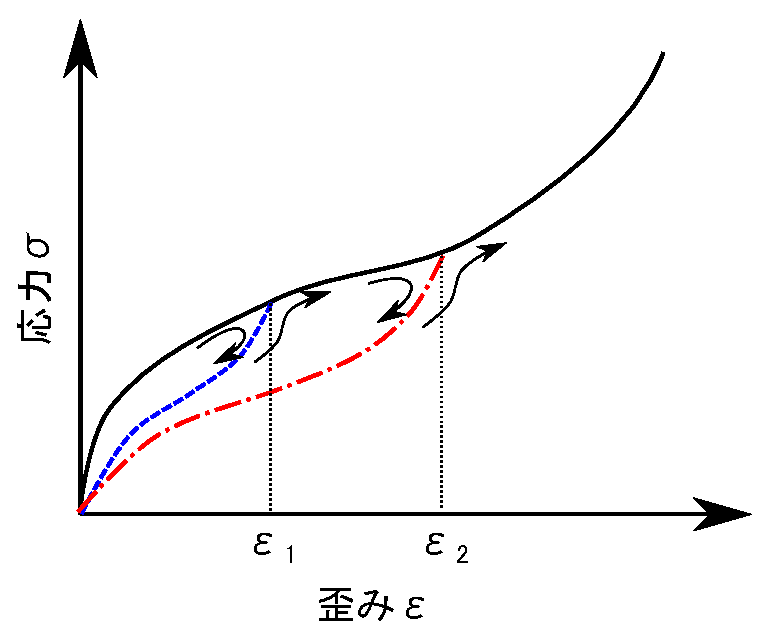
\includegraphics[width=35mm]{Mullins_Efct.eps}
% \end{columns}

% \end{frame}
    
% \begin{frame}
% \frametitle{ターゲット}


% 破壊耐性に優れた軽量材料の候補として「ゴム材料」を選択

% \begin{alertblock}{設計のポイント}
% \begin{itemize}
% \item
% 可逆性の有効利用
%     \begin{itemize}
%     \item
%     可逆性の高いヒステリシスの設計
%     \end{itemize}
%     \item 弾性限界の設計
%     \begin{itemize}
%     \item
%     伸びきり効果の明確化
%     \end{itemize}
% \end{itemize}
% \end{alertblock}

% \Large
% 物性設計のために、\\「構造明確なネットワーク」が必要
% \end{frame}
    
\begin{frame}

\frametitle{構造の明確なネットワーク}

\begin{alertblock}{構造の明確なネットワーク}
\begin{itemize}
\item 設計方針が明確となり、フィードバックが容易。
\item 基盤技術の見極めに適する。
\end{itemize}

\end{alertblock}


\begin{block}{二つの具体的アプローチ}
Tetra-PEG gel
    \begin{itemize}
    \item
    末端官能性四本鎖
    \item
    均質なネットワーク構造を有するゲルを形成
    \end{itemize}

超分子ネットワーク
    \begin{itemize}
    \item
    「繋ぎ替え可能な非共有結合(水素結合、疎水性相互作用…)」を介して自己組織化
    \item
    無溶剤での構造の明確なネットワークの形成
    \end{itemize}
\end{block}
\end{frame}
    
\begin{frame}
%[shrink squeeze]
%[allowframebreaks]
\frametitle{超分子ネットワークの固定化}

ESA-CF 法 (Electrostatic Self-assembly and Covalent Fixation)\\
{\scriptsize Y. Tezuka, E.J. Goethals, European Polymer Journal, 991, 1982}

\begin{itemize}
\item
両末端に開環反応性アンモニウム塩を有する\\テレケリックアイオノマー
\begin{itemize}
\item
両末端トリフラート型ポリ THF (カチオン開環重合)
\item
環状三級アミンと反応(ドーマント種に変換)
\end{itemize}
\item
\alert{多価カルボン酸との塩交換により超分子ネットワークを形成}
\item<2>
\alert{加熱により以下の反応で共有結合へと変換}
\end{itemize}

\centering
    \includegraphics<1>[width=5cm]{Network_2.pdf}

    \includegraphics<2>[width=5cm]{Network_2_linked.pdf}

\end{frame}
    

\begin{frame}
\frametitle{可逆反応+共有結合への変化での固定化}

\begin{block}{組み換え可能な可逆反応の利用}

\begin{itemize}
    \item
    応力によるつなぎ替えが可能な可逆反応
    \begin{itemize}
        \item
        ネットワークトポロジーの最適化
        \item
        接着時に発生した応力も緩和可能 \\⇒ 迅速な増粘後にゆっくり緩和
    \end{itemize}
\end{itemize}
\end{block}

\vspace{-8mm}
\begin{center}
\LARGE{+}
\end{center}
\vspace{-5mm}

\begin{alertblock}{共有結合への変化による固定化}
    \begin{itemize}
        \item
        クリープ抑制のために
        \begin{itemize}
            \item
            適切な時間経過後に、共有結合に変化
            \item
            適正なトポロジーを維持
        \end{itemize}	
    \end{itemize}
\end{alertblock}
\end{frame}
    
    % %%%%%
    % \subsection{本研究の目標とアプローチ}
    % \begin{frame}
    % %[shrink squeeze]
    % %[allowframebreaks]
    % \frametitle{本研究の目標とアプローチ}
    % \begin{exampleblock}{本研究の目標とアプローチ}
    % \begin{itemize}
    % \item
    % 目標\\
    % 破壊耐性に優れた軽量材料の創成とその設計指針の明確化
    % \item
    % アプローチ
    %     \begin{itemize}
    %     \item
    %     可逆性に優れた材料としてゴム材料を選択。
    %     \item
    %     構造明確なネットワークの構築のために超分子ネットワーク。
    %     \item
    %     既知のモデルとの整合性を確認。
    %     \item
    %     シミュレーションの併用でマルチスケールモデルを構築
    %     \end{itemize}
    % \end{itemize}
    % \end{exampleblock}
    
    
    % \begin{block}{本発表の内容}
    % 本発表では、反応性テレケリックアイオノマーを用いた超分子ネットワークの特性について概観したのちに、熱架橋により得られたエラストマーの力学特性評価を行った結果について報告を行う。
    % \end{block}
    
    % \end{frame}
    
    % %%%%%
    % \section{テレケリックアイオノマー・ネットワークの特性}
    % %%%%%
    % \begin{frame}
    % \LARGE{テレケリックアイオノマー・ネットワークの特性}
    % \end{frame}
    
    % %%%%%%%%%%%
    % \subsection{テレケリックアイオノマー・ネットワークの合成}
    % %%%

\begin{frame}
    \frametitle{テレケリックアイオノマーの検討結果}
    
    ESA-CF 法 (Electrostatic Self-assembly and Covalent Fixation)\\による超分子ネットワーク\\
    {\scriptsize Y. Tezuka, E.J. Goethals, European Polymer Journal, 991, 1982}
    
    \begin{columns}[T, totalwidth=\linewidth]
    \column{.32\linewidth}
        {\scriptsize テレケリックアイオノマーの合成}
        \includegraphics[width=\columnwidth]{Telechelic_Anion_2.png}
        
        {\scriptsize ネットワークイメージ}
        %\vspace{3mm}
        \includegraphics[width=\columnwidth]{Network_2.pdf}
    \column{.32\linewidth}<2->
        {\scriptsize 
        レオメータで、温度ジャンプにより反応性を評価
        \begin{itemize}
        \item
        疑一次反応で架橋反応を記述可能
        \item
        付加反応は反応律速
        \item
        塩構造の末端基がクラスタを形成?
        \end{itemize}
        }
        \includegraphics[width=\columnwidth]{Cure_100deg.pdf}
    \column{.32\linewidth}<3>
        {\scriptsize
        形成ネットワークの力学特性
        \begin{itemize}
        \item
        古典ゴム理論で、伸長特性を記述可能
        \item
        C2 の寄与が比較的大きい
        \item
        伸び切り効果が顕著
        \end{itemize}
        }
        \includegraphics[width=\columnwidth]{SS_wMR_5_2.pdf}
    \end{columns}
\end{frame}

% \begin{frame}
% \frametitle{具体的な合成反応}

% ポリマーの両末端にカチオン開環性官能基を有するテレケリックアイオノマーネットワークの合成\\
% {\scriptsize Y. Tezuka, E.J. Goethals, European Polymer Journal, 991, 1982}

% \begin{columns}[totalwidth=\textwidth]
% \column{.5\textwidth}
% \begin{itemize}
% \item
% テレケリックアイオノマーの合成
%     \begin{itemize}
%     \item
%     リビングカチオン重合で両末端トリフラート型ポリ THF
%     \item 
%     さらに、五員環のフェニルピロリジンと反応
%     \end{itemize}
% \end{itemize}
% \centering
% \includegraphics[width=.6\textwidth]{Telechelic_Anion_2.png}
% \column{.5\textwidth}
% \begin{itemize}
% \item
% 超分子ネットワークの形成
%     \begin{itemize}
%     \item
%     三官能のトリメリット酸で塩交換
%     \item
%     溶剤流去、乾燥 $\rightarrow$ シート形状の超分子ネットワーク
%     \end{itemize}
% \end{itemize}
% \centering
% \includegraphics[width=.6\textwidth]{Network_2.pdf}

% \end{columns}
% \end{frame}

\begin{frame}
    \frametitle{ここまでのまとめ}

    \begin{boxnote}
        \begin{itemize}
            \item 院試をきっかけに、\alert{「広範な知識を関係づけることの重要性」}を実感。
            \item Synchronicity(意味のある偶然の一致)は結構生じる。
            \item 目の前のチャンスを逃さない。
            \item 落穂拾いは役に立つ。
            \begin{itemize}
                \item オキセタンの再発見 1960-
                \item ゴムの強靭性 1960-
                \item 超分子ネットワーク 1990-
            \end{itemize}
        \end{itemize}
    \end{boxnote}

\end{frame}

\section{考えてきたこと}
\subsection{モデル化による現象の理解}
\begin{frame}
    \frametitle{モデル化による現象の理解}
    \note[item]{あくまでも、化学系出身の私にとってなんですが、物理系では当たり前の、「自然現象の背後にあるユニバーサリティーの理解と、適正なレベルでのモデル化」という考え方がかけていました。}
    \note[item]{自身の周りを振り返りますと、}

    \begin{block}{化学系企業でありがちな状態}
        \begin{itemize}
            \item 教科書的なものの背後にある物理的、数学的な思想を理解することからの逃避
            \item 数式や物理モデルの盲目的な受認によるデータの処理
            \item 統計的な妥当性の確認の放棄
            \item 客観的な視点に基づく独立事象と従属事象の切り分けの放棄
        \end{itemize}
    \end{block}

    \begin{alertblock}{化学系の人間としての過去の自身に欠けていたもの}
        \begin{itemize}
            \item 物理系では当たり前の考え方
            \begin{itemize}
                \item 自然現象の背後にあるユニバーサリティーの理解
                \item 適正なレベルでのモデル化
            \end{itemize}
        \end{itemize}
    \end{alertblock}
\end{frame}

\begin{frame}
    \frametitle{最近の風潮}
            \begin{block}{直ぐに結果を求めたがる}
                \begin{itemize}
                    \item 実事象はあまりに複雑で因果関係がわかりにくいのに、すぐに結果を求める。
                    \begin{itemize}
                        \item 具体的な対策、方法論を望む
                        \item 考え方の提示では満足しない
                    \end{itemize}
                    \item シミュレーションに対しても考え方の指針ではなく、\\答えを求める。
                    \begin{itemize}
                        \item 概念的なものをあまり重視しない。
                        \item そのようなアプローチは、汎用性を生み出さない。
                    \end{itemize}
                \end{itemize}

                    \centering
                        \includegraphics[width=.4\textwidth]{usagi_kame.jpg}
                
            \end{block}
\end{frame}

\subsection{化学と物理}
\begin{frame}
    \frametitle{化学と物理を比べると}
    \note[item]{化学系の人は、基本的には天下りを受容しがちかと思います。}
    \note[item]{これは有り様を実感できない分子、原子を対象とするため、見えないものを受け入れる}
    \note[item]{一方、これはいいことなんですが、多様性を容認するという雰囲気があります。}
    \note[item]{自由エネルギー、平衡状態、定常状態、等の熱力学の基本が曖昧な場合も多い。}
    \note[item]{ちょっとイチャモンかもしれませんが、偏微分でビビる人が多いのかもしれません}
    \begin{columns}[T, onlytextwidth]
        \column{.48\linewidth}
        \begin{block}{化学のやり方}
            \begin{itemize}
                \item 基本的に天下りを受容
                \begin{itemize}
                    \item 実感できない分子、原子を対象
                    \item 見えないものを受容
                    % \item 「誰が原子を見たか」
                \end{itemize}
                \item 多様性を容認
                \item 熱力学が理解できていない人が、けっこう多い
            \end{itemize}

                \centering
                    \includegraphics[width=.36\textwidth]{chem_frog.png}
            
        \end{block}
        
        \column{.48\linewidth}
        \note[item]{化学系出身の私には、隣の芝生は青いと見えているのかもしれませんが、物理的な考え方は、理論の筋道をきちんと捉えようとしていると感じます。}
        \note[item]{まあ、私がフォーカスしているソフトマター関連の感覚かもしれませんが。} 
        \note[item]{これは、エイヤと私が感心したものを並べただけですが。}
        \begin{exampleblock}{物理的な考え方}
            \begin{itemize}
                \item 事象に内在する一般性
                \item その本質に迫るために\\モデル化
                \item 興味深い考え方:\\
                揺動散逸定理、線形応答理論、臨界現象、スケーリング則、無次元化
            \end{itemize}

            \centering
            \includegraphics[width=.32\textwidth]{phys_frog.png}
        \end{exampleblock}  
    \end{columns}
\end{frame}

% \begin{frame}
%     \frametitle{ソフトマターでの印象派物理}
%     \note[item]{ソフトマターでは、結構自由な考え方があります。これをほんのタイトルにしたのは御茶ノ水の奥村先生ですが、まあ、以前からあるような流れかと思います。}
%     \begin{itemize}
%         \item 印象派とは数学的な詳細をあえて大胆に無視することでシンプルに捉え、本質に迫るスタイルのこと
%         \item 写実主義的物理との対比
%         \item P-G de Gennes からのフランスでの潮流
%         \item まわりの実験家とつねに対話をして、身の回りの事象に対して強い好奇心を持ち、斬新なアイデアを創出
%         \item 大胆な発想での理解;「大いなる同一視」
%     \end{itemize}
% \end{frame}

\subsection{抽象的と具体的}
\begin{frame}
    \frametitle{抽象的に考える}
    \note[item]{少し話は変わってきますが、抽象的に考えるということについてです。会社の人の中には、抽象的という言葉に否定的なことも多いかと感じます。}
        \begin{itemize}
            \item 抽象的ということを非現実的と捉え、「えそらごと」と読んでしまう人のなんと多いことか。
        \end{itemize}
    \begin{exampleblock}{抽象とは}
        「抽象」という語については、「事物や表象からある性質・共通性・本質を抽(ひ)き出して把握する」つまり「象を抽き出す」という意味を持つ語
        \begin{itemize}
            \item 個々の事物の本質・共通の属性を抜き出して、\alert{一般的な概念をとらえる}さま。
            \item 単に概念的に思考されるだけで、実際の形態・内容を持たないさま。
        \end{itemize}
        \textcolor{blue}{後者の意味の反意語は、具体的}
    \end{exampleblock}
    \large{\alert{抽象化は、モデル化に必須。}}
\end{frame}



\begin{frame}
    \frametitle{単純化して概念へと昇華する方法論}

            \begin{exampleblock}{抽象と捨象}
                \begin{itemize}
                    \item 捨象は捨てる行為に、フォーカスする。
                    \item 単純化する際に、抽き出す行為と捨てる行為
                    \item どちらも不要なものに埋もれた中から、\\本質につながる単純化
                    \item 粗視化はどちらであるべきか?
                    \item<2> 高校時代の美術の熊井先生の\alert{走り回り画法}
                    \begin{itemize}
                        \item<2> 目を細めて対象物を眺め、ディーテールを無視して、\\目に留まる主要な色を用いて下書き
                        \item<2> 全体に共通なトーンや色合いの部分を、\\\alert{全体に筆を走り回らせ}ながら書き込む。
                        \item<2> 段階的に、微細なディーテールへと
                    \end{itemize}
                \end{itemize}
            \end{exampleblock}
\end{frame}

\section{私のおすすめ}
\subsection{感じてきたこと}
\begin{frame}
	\frametitle{感じてきたこと}
		\begin{alertblock}{これまでの経験を通して感じてきたこと}
			\begin{itemize}
				\item 「化学をベースに、尤もらしく」
				\begin{itemize}
					\item 「新規なものを作り出す技術としての\alert{化学の有用性}」
					\item \textcolor{blue}{経験則を重視して、個別の理由を考えがち。}
					\item \textcolor{blue}{化学構造式で物質を設計しようとしがち}
				\end{itemize}
				\item 「物理、数学、統計の考えを利用して」
				\begin{itemize}
					\item 「\alert{事象を客観視し、普遍性を大事}にする考え方」
					\item 雑多な化学の中に\alert{シンプルな論理性を}
				\end{itemize}
				\item 「できるだけシンプルなモデルで。」
				\begin{itemize}
					\item 数学や物理で用いられる\alert{モデル化が非常に有用}
					\item 適切なモデル化で、尤もらしいストーリーを構築
				\end{itemize}
			\end{itemize}
		\end{alertblock}
\end{frame}

% \subsection{考え方のコツ}
\begin{frame}
	\frametitle{考え方のコツ}
		\begin{block}{感じてきたことをまとめ直すと、}
			\begin{itemize}
				\item 化学構造式と実際の物性の関係は非常に複雑。
				\begin{itemize}
					\item ややこしいものを、全部理解しようとしても無理。
					\item かと言って、単純化しすぎても役に立たない。
				\end{itemize}
				\item 「なぜそうなっているんだろう?」と考えてみる。
				\begin{itemize}
					\item 自分の言葉で理由を考えて、
					\item 人に説明できるように話の流れを作る。
					\item 流れの各ステップはできるだけ単純に。
				\end{itemize}
				\item できるだけシンプルな実験を
				\begin{itemize}
					\item 同時に仮定を複数設定しないこと。
					\item 実験前によく考えて計画を建てる。
					\item 一つずつ検証していく。
				\end{itemize}
			\end{itemize}
		\end{block}
\end{frame}

\subsection{MIへの違和感}
\begin{frame}
    \frametitle{MI への違和感}
    \note[item]{まあ、これは、私の勝手な偏見に基づくものかなとは思っているのですが、MIに対してはかなり違和感を持っております。}
    \note[item]{機械学習に関しては、特定の分野では非常に有効だろうなとは感じております。}
    \note[item]{悪口ばかりでも何なんで、使い方次第とは思います。}
    \note[item]{例えば、ランダムフォレスト等を用いて、説明変数や目的変数の交絡状態を評価したりすること自体は有用かと。}
    \note[item]{でも、やはり、統計モデリングと言われるような手法と、MIとは、なんだか色合いが異なるように感じるのです。}
    \note[item]{これは、嗜好の問題なんでしょうけれど、物理的に意味を持つモデリングを形成することこそが、後の展開を広げられるのではないかと。}
    \note[item]{昨日の実験科学のセッションの発表でも、物理的に意味を持つような説明変数や目的変数をうまく見つけ出して、その因果関係を納得できる道筋でつなげていくことが大事なのかなと感じるのです。}
    \note[item]{この辺の感覚は、先日、講演をお聞きした九大の廣瀬准教授のアプローチには納得するものがあったことはお伝えしておきます。}
    \begin{block}{機械学習について}
        機械学習は特定の分野では非常に有効
        \begin{itemize}
            \item 回帰的手法をベースとした多変量解析
            \item 自動運転のようなフィードバック系
        \end{itemize}
    \end{block}
    \begin{exampleblock}{MI への違和感}
        
        \begin{itemize}
            \item (一部の方に見られる)思考を放棄したような無手勝流
            \item 少なくとも、MI を打ち出の小槌と捉えてはいけない。
            \item シミュレーションを実験の代替とする方法論は有効。
            \item 考えるための道具として有効活用すべき。
            \item 因果推論も確からしくできるようになってきたらしい
        \end{itemize}
    \end{exampleblock}
\end{frame}

\begin{frame}
    \frametitle{基礎知識の汎用化について}
        \begin{exampleblock}{データサイエンスの企業での使いこなし}
            \begin{itemize}
                \item データサイエンティストの中途採用
                \begin{itemize}
                    \item マネージメントの難しさ $\Rightarrow$ プロの持ち腐れ
                    \item 現役データサイエンティストの満足度は低い
                    \begin{itemize}
                        \item 手本がない
                        \item 周りの理解がない
                        \item スキルアップの時間がない
                    \end{itemize}
                \end{itemize}
            \end{itemize}
        \end{exampleblock}
        \begin{alertblock}{「データサイエンスの民主化」}
            \begin{itemize}
                \item 文系、数学苦手は関係ない
                \item データをもとに客観的に考えるという基本的な概念
                \item 関係者みんなに広く浅く(深いに越したことはない)
            \end{itemize}
        \end{alertblock}
        \centering
        \Large{\alert{研究一般についても大事}}
\end{frame}

\begin{frame}
    \frametitle{あるべき状態}
    \begin{exampleblock}{化学系研究者の立ち位置}
        \begin{itemize}
            \item 試行錯誤ベースで実際に物質を合成することは必須
            \item 物理側からの理論的な成果を盲目的に受容しては駄目
        \end{itemize}
    \end{exampleblock}
    \begin{alertblock}{あるべき状態}
        \begin{itemize}
            \item 物理的な思考による事象の成り立ちの理解、および、モデル化への道すじを共有
            \item 目的を明確にし、適切な次元、スケール及び時間軸で、議論を行う
            \item 物質の多様性を前提とした化学的な方法論の整理と、適正なモデル化への挑戦
            \item 物理及び化学双方の方法論についての\alert{相互理解の深化}
        \end{itemize}
    \end{alertblock}
\end{frame}


\subsection{私のやり方}

\begin{frame}
	\frametitle{自分の中への落とし込み}
		\begin{block}{「何のためにやりたいのか?」を明確に}
			\begin{itemize}
				\item 目的がわからないと、ゴールが見えてこない。
				\item 仕事であれば、上司とよく相談すること。
				\item 自己啓発であれば、自分の本心をよく見極める。
			\end{itemize}
		\end{block}
		\pause
		\begin{block}{「何をやりたいのか?」を常に意識}
			\begin{itemize}
				\item 因果関係をはっきりと。
				\begin{itemize}
					\item 因 $\Leftarrow$ 原因
					\item 果 $\Leftarrow$ 結果
				\end{itemize}
				\item 図として書下せるように理解する。
				\begin{itemize}
					\item 複雑な実事象をできるだけ単純化して、
					\item 一目で理解できるようにすることが大事。
				\end{itemize}
			\end{itemize}
		\end{block}
\end{frame}

\begin{frame}
	\frametitle{色々なモデル化}
	「さまざまな条件のもとで、幅広い検討対象に対してでも当てはめることのできるような汎用的なモデル」を考えることが役にたったと実感。
	\begin{exampleblock}{モデル化のすすめ}
		\begin{columns}[c, onlytextwidth]
			\column{.68\linewidth}
			\begin{itemize}
				\item 適度な深さで尤もらしく
					\begin{itemize}
						\item 簡単すぎるものは例外が多い。
						\item 複雑化しすぎても過適応
							\begin{itemize}
								% \item n個のデータを、n次の関数でフィット
								\item 個々の現象にだけ適応可能
								\item モデル化する意味がない
							\end{itemize}
					\end{itemize}
				\item 欲しいもの
					\begin{itemize}
						\item 汎用的に使えるモデル
						\item 尤もらしく、実験事実を説明可能
					\end{itemize}
			\end{itemize}
			\column{.3\linewidth}
					\centering
						\includegraphics[width=\textwidth]{souzou.png}
		\end{columns}
	\end{exampleblock}
\end{frame}

% \subsection{目指すもの}

\begin{frame}
	\frametitle{おすすめのやり方}
	
	\begin{center}
		{\Huge \textbf{「急がば回れ」}}
	\end{center}
	
	\vspace{5mm}
	\begin{alertblock}<2->{ざっくり全体像をイメージ}
		\begin{columns}[c, onlytextwidth]
			\column{.6\linewidth}
			\begin{itemize}
				\item 慌てて結果を出そうとしない。
				\begin{itemize}
					\item 心を落ち着けて、
					\item やるべきことを、
					\item 明確にイメージする。
				\end{itemize}
				\item 全体像をザックリと捕まえる。
				\item 理解は一気に容易になり、
				\item ゴールへの道も見えてくる。
			\end{itemize}
			\column{.35\linewidth}
					\centering
						\includegraphics[width=\textwidth]{goal.png}
		\end{columns}
	\end{alertblock}
\end{frame}

% \begin{frame}
%     \frametitle{私のやり方}
%         \begin{itemize}
%             \LARGE
%             \item 急がば回れ
%             \begin{itemize}
%                 \Large
%                 \item<2-> 慌ててやっても無駄
%                 \item<2-> ゆっくりキチンと組み立てる
%             \end{itemize}
%             \item 備えよ常に
%             \begin{itemize}
%                 \Large
%                 \item<3-> 見えないものにも前もって
%                 \item<3-> 泥縄にならないように
%             \end{itemize}
%             \item 腑に落とす(落ちる)
%             \begin{itemize}
%                 \Large
%                 \item<4> 消化して使いこなす
%                 \item<4> 頭でっかちにならない
%             \end{itemize}
%         \end{itemize}
% \end{frame}

\begin{frame}
    \frametitle{他人の意見について}
        \begin{columns}[c, onlytextwidth]
            \column{.54\linewidth}
            \large
            \begin{block}{その道のプロの言うこと}
                \begin{itemize}
                    \large
                    \item それなりの確からしさ
                    \item 前提条件の確認が必要
                    \begin{itemize}
                        \large
                        \item 常識が異なる
                        \item 暗黙の了解が多数
                    \end{itemize}
                    \item 素人が下手に使う怖さ
                \end{itemize}
            \end{block}
            \column{.02\linewidth}
            \column{.44\linewidth}<2-3>
            \LARGE
                \alert{「盲目的に\\信じてはだめ」}
        \end{columns}
    \begin{alertblock}<3>{腑に落とす(落ちる)}
        \begin{itemize}
            \item<3> 消化して使いこなす
            \item<3> 頭でっかちにならない
        \end{itemize}
    \end{alertblock}
        
\end{frame}

\begin{frame}
    \frametitle{自分の頭で考える}
        \begin{alertblock}{胃の腑に落とすということは?}
            無理やり胃に落としてもだめ!!
        \end{alertblock}

        % \vspace{-3mm}
        \begin{columns}[T, onlytextwidth]
            \column{.48\linewidth}
            
            \begin{block}{咀嚼するための基礎学力}
                STEAM 
                \begin{itemize}
                    \item Science
                    \item Technology
                    \item Engineering
                    \item \alert{Art}
                    \begin{itemize}
                        % \item<2> 体系立てて捉える
                        \item<2-> 成り立ちの美しさ
                        \item<2-> 哲学的な統一性 
                    \end{itemize}
                    \item Mathematics
                \end{itemize}
            \end{block}
            \column{.48\linewidth}
                \centering
                    \includegraphics<1-2>[width=\textwidth]{steam.png}

                    % \footnotesize{https://steam-japan.com/about/}
                    \begin{exampleblock}<3>{消化(使いこなす)ために?}
                        \begin{itemize}
                            \item 特定分野に囚われない広範な知見
                            \item 締め切りを決めない
                            \item ゆっくり考える
                            \item 自由な議論
                            \item 数値化にこだわらない
                            \item 目に見えないものを\\大事に
                        \end{itemize}
                    \end{exampleblock}
        \end{columns}
\end{frame}

% \begin{frame}
%     \frametitle{自分の頭で考える}
%         \begin{alertblock}{胃の腑に落とすということは?}
%             無理やり胃に落としてもだめ!!
%         \end{alertblock}
%         \begin{columns}[T, onlytextwidth]
            
%             \column{.48\linewidth}  
%             \vspace{-3mm}
%             \begin{block}{咀嚼するための基礎学力}
%                 STEAM 
%                 \begin{itemize}
%                     \item Science
%                     \item Technology
%                     \item Engineering
%                     \item \alert{Art}
%                     \begin{itemize}
%                         % \item<2> 体系立てて捉える
%                         \item 成り立ちの美しさ
%                         \item 哲学的な統一性 
%                     \end{itemize}
%                     \item Mathematics
%                 \end{itemize}
%             \end{block}
            
%             \column{.48\linewidth}
%             \vspace{-3mm}
%             \begin{exampleblock}{消化(使いこなす)ために?}
%                 \begin{itemize}
%                     \item 特定分野に囚われない広範な知見
%                     \item 締め切りを決めない
%                     \item ゆっくり考える
%                     \item 自由な議論
%                     \item 数値化にこだわらない
%                     \item 目に見えないものを\\大事に
%                 \end{itemize}
%             \end{exampleblock}
%         \end{columns}
% \end{frame}

\begin{frame}
    \frametitle{まとめに代えて}
        \begin{exampleblock}{私のアプローチ}
            \begin{itemize}
                \item 自由に議論できる場の創設
                \begin{itemize}
                    \item Slack を利用して、「東海ソフトマター」を設置
                    \item 大学、企業半々程度の参加者
                    \item それをベースに、Web会議で「ザツダン会」を開催
                \end{itemize}
                \item 基本的な知見の再整理
                \begin{itemize}
                    \item Moodle システムを利用して、LMSサイトを整備中
                    \item 自身の初心者としての疑問点にフォーカスして整理
                    \item 対象:レオロジー、高分子物理、統計等
                \end{itemize}
                \item 定年後のセミナー会社
                \begin{itemize}
                    \item 上記の基礎的な事項に関するセミナー、オンデマンド
                    \item 学生は無料
                \end{itemize}
            \end{itemize}
        \end{exampleblock}
\end{frame}


\end{document}
